% slides_disco_interview.tex
% DISCO Corporation — 2nd-round interview slide deck
% Build: pdflatex -interaction=nonstopmode slides_disco_interview.tex  (twice)
\documentclass[aspectratio=169,10pt]{beamer}

\usetheme{Boadilla}
\usecolortheme{crane}

\usepackage{lmodern}
\usepackage[T1]{fontenc}
\usepackage[utf8]{inputenc}
\usepackage{amsmath,amssymb}
\usepackage{booktabs}
\usepackage{graphicx}
\usepackage{xcolor}
\usepackage{tikz}
\usetikzlibrary{arrows.meta,positioning,fit,shapes.geometric,backgrounds}
\usepackage{listings}
\usepackage{hyperref}
\usepackage{multirow}

% ── colours ──────────────────────────────────────────────────────────────
\definecolor{disco_navy}{RGB}{0,51,102}
\definecolor{disco_gold}{RGB}{180,140,0}
\definecolor{disco_light}{RGB}{230,240,255}

% ── metadata ─────────────────────────────────────────────────────────────
\title[SiC Dicing Simulation]{SiC Dicing Process Simulation\\
  \& AI-Driven Recipe Optimisation}
\subtitle{DISCO Corporation --- 2nd Interview}
\author{Keisuke Nishioka}
\institute{Leibniz University Hannover / SFB TRR-298}
\date{2026}

% ── helper: block-quote style ────────────────────────────────────────────
\newcommand{\kv}[2]{\textbf{#1}: #2}

% ── listing style ────────────────────────────────────────────────────────
\lstset{
  basicstyle=\ttfamily\tiny,
  breaklines=true,
  frame=single,
  backgroundcolor=\color{disco_light},
  rulecolor=\color{disco_navy},
}

% ─────────────────────────────────────────────────────────────────────────
\begin{document}

% ── 1. TITLE SLIDE ───────────────────────────────────────────────────────
{
\setbeamertemplate{footline}{}
\begin{frame}[plain]
  \titlepage
  \vspace{-1em}
  \begin{center}
    \small
    \textcolor{disco_navy}{%
      FEM $\to$ GP Surrogate $\to$ PAT $\to$ DDPM $\to$ DeepONet}
  \end{center}
\end{frame}
}

% ── 2. DISCO BUSINESS UNDERSTANDING ──────────────────────────────────────
\begin{frame}{DISCO Business Understanding}
  \begin{columns}[T]
    \begin{column}{0.48\textwidth}
      \textbf{4H-SiC Dicing --- Key Engineering Facts}
      \vspace{0.5em}

      \begin{itemize}
        \item \kv{Spindle}{PMSM air-bearing spindle, 60{,}000~rpm}
        \item \kv{Stage}{XY linear servo, sub-$\mu$m positioning}
        \item \kv{Blade}{Resin/metal-bond diamond, 50--200~$\mu$m thick}
        \item \kv{SiC hardness}{$9.5$ Mohs, anisotropic fracture on\\
              $\{0001\}$ basal + $\{10\bar{1}0\}$ prism planes}
      \end{itemize}

      \vspace{0.8em}
      \textbf{Why SiC? --- Market Drivers}
      \begin{itemize}
        \item EV power modules: 650--1200~V SiC MOSFET demand\\
              $\times 3$ by 2028 (Yole forecast)
        \item 6-inch $\to$ 8-inch migration: tighter chipping spec ($<5~\mu$m)
        \item Device yield is process-yield; dicing quality is\\
              directly on the critical path
      \end{itemize}
    \end{column}
    \begin{column}{0.48\textwidth}
      \centering
      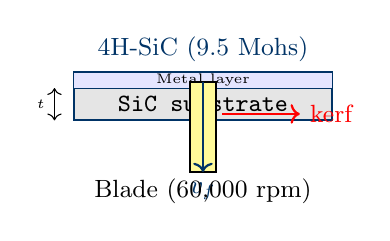
\begin{tikzpicture}[scale=0.82, font=\small]
        % Wafer cross-section schematic
        \draw[fill=gray!20, draw=disco_navy, thick]
          (0,0) rectangle (4,0.5) node[midway]{\texttt{SiC substrate}};
        \draw[fill=blue!10, draw=disco_navy]
          (0,0.5) rectangle (4,0.75) node[midway]{\tiny Metal layer};
        % Blade
        \draw[fill=yellow!40, draw=black, thick]
          (1.8,-0.8) rectangle (2.2,0.6);
        \draw[->, thick, disco_navy] (2,0.6) -- (2,-0.8)
          node[below]{\small $v_f$};
        \draw[->, thick, red] (2.3,0.1) -- (3.5,0.1)
          node[right]{\small kerf};
        % Labels
        \node at (2,-1.1) {\small Blade (60{,}000 rpm)};
        \node[text=disco_navy] at (2,1.1)
          {\small 4H-SiC ($9.5$ Mohs)};
        \draw[<->,thin] (-0.3,0) -- (-0.3,0.5)
          node[left,midway]{\tiny $t$};
      \end{tikzpicture}

      \vspace{1em}
      \begin{block}{DISCO's edge}
        \small
        DFD\textsuperscript{\textregistered} (stealth dicing) + Kabra\textsuperscript{\textregistered} (laser):
        DISCO controls $>$60\% of global dicing tool market.
      \end{block}
    \end{column}
  \end{columns}
\end{frame}

% ── 3. RESEARCH OVERVIEW (BLOCK DIAGRAM) ─────────────────────────────────
\begin{frame}{Research Overview --- Five Modelling Modules}
  \centering
  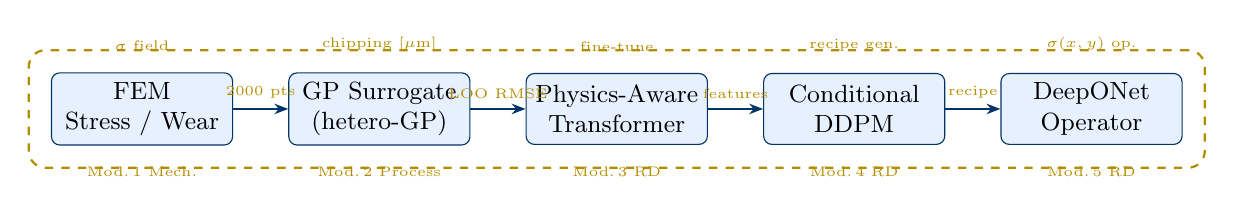
\begin{tikzpicture}[
      node distance=0.5cm and 0.7cm,
      box/.style={draw=disco_navy, fill=disco_light, rounded corners=3pt,
                  minimum width=2.3cm, minimum height=0.9cm,
                  align=center, font=\small},
      arr/.style={-{Stealth[length=5pt]}, disco_navy, thick},
      lbl/.style={font=\tiny, text=disco_gold},
    ]
    \node[box] (fem)   {FEM\\Stress / Wear};
    \node[box, right=of fem]  (gp)  {GP Surrogate\\(hetero-GP)};
    \node[box, right=of gp]   (pat) {Physics-Aware\\Transformer};
    \node[box, right=of pat]  (ddpm){Conditional\\DDPM};
    \node[box, right=of ddpm] (dop) {DeepONet\\Operator};

    \draw[arr] (fem)  -- node[lbl,above]{2000 pts} (gp);
    \draw[arr] (gp)   -- node[lbl,above]{LOO RMSE} (pat);
    \draw[arr] (pat)  -- node[lbl,above]{features} (ddpm);
    \draw[arr] (ddpm) -- node[lbl,above]{recipe} (dop);

    % second row: roles
    \node[lbl, below=0.15cm of fem]  {Mod.\,1 Mech.};
    \node[lbl, below=0.15cm of gp]   {Mod.\,2 Process};
    \node[lbl, below=0.15cm of pat]  {Mod.\,3 RD};
    \node[lbl, below=0.15cm of ddpm] {Mod.\,4 RD};
    \node[lbl, below=0.15cm of dop]  {Mod.\,5 RD};

    % top row: target spec
    \node[lbl, above=0.15cm of fem]  {$\sigma$ field};
    \node[lbl, above=0.15cm of gp]   {chipping $[\mu$m]};
    \node[lbl, above=0.15cm of pat]  {fine-tune};
    \node[lbl, above=0.15cm of ddpm] {recipe gen.};
    \node[lbl, above=0.15cm of dop]  {$\sigma(x,y)$ op.};

    % outer bounding box
    \begin{pgfonlayer}{background}
      \node[draw=disco_gold, dashed, thick, rounded corners=6pt,
            fit=(fem)(dop), inner sep=8pt] {};
    \end{pgfonlayer}
  \end{tikzpicture}

  \vspace{0.8em}
  \begin{columns}[T]
    \begin{column}{0.32\textwidth}
      \small
      \textbf{Data:} $n=11$ Grade-A experimental cuts\\
      (varied feed $v_f$, depth $a_p$, rpm $n_s$)
    \end{column}
    \begin{column}{0.32\textwidth}
      \small
      \textbf{Physics:} 4H-SiC anisotropy,\\
      MRR, SFR, Hertzian contact model
    \end{column}
    \begin{column}{0.32\textwidth}
      \small
      \textbf{Goal:} chipping $< 5~\mu$m,\\
      recipe auto-generation, stress field
    \end{column}
  \end{columns}
\end{frame}

% ── 4. GP SURROGATE ──────────────────────────────────────────────────────
\begin{frame}{Process --- GP Surrogate for Chipping Prediction}
  \begin{columns}[T]
    \begin{column}{0.52\textwidth}
      \textbf{Heteroscedastic Gaussian Process}
      \begin{itemize}
        \item Input: $(v_f, a_p, n_s)$; output: lateral chipping $[\mu\text{m}]$
        \item Noise variance fitted per observation\\
              (process noise $\neq$ const at high feeds)
        \item Kernel: Mat\'ern-5/2 + white noise
        \item LOO cross-validation: \textbf{RMSE = 1.62~$\mu$m}\\
              on $n = 11$ Grade-A experimental points
      \end{itemize}

      \vspace{0.5em}
      \begin{block}{Why GP?}
        \small
        Uncertainty quantification $\Rightarrow$ safe active-learning
        next-experiment selection (EI acquisition).\\
        New recipe candidates ranked before cutting.
      \end{block}

      \vspace{0.5em}
      \texttt{ml/gp\_experimental.py}\\
      \texttt{results/gp\_experimental.pkl}
    \end{column}
    \begin{column}{0.44\textwidth}
      \centering
      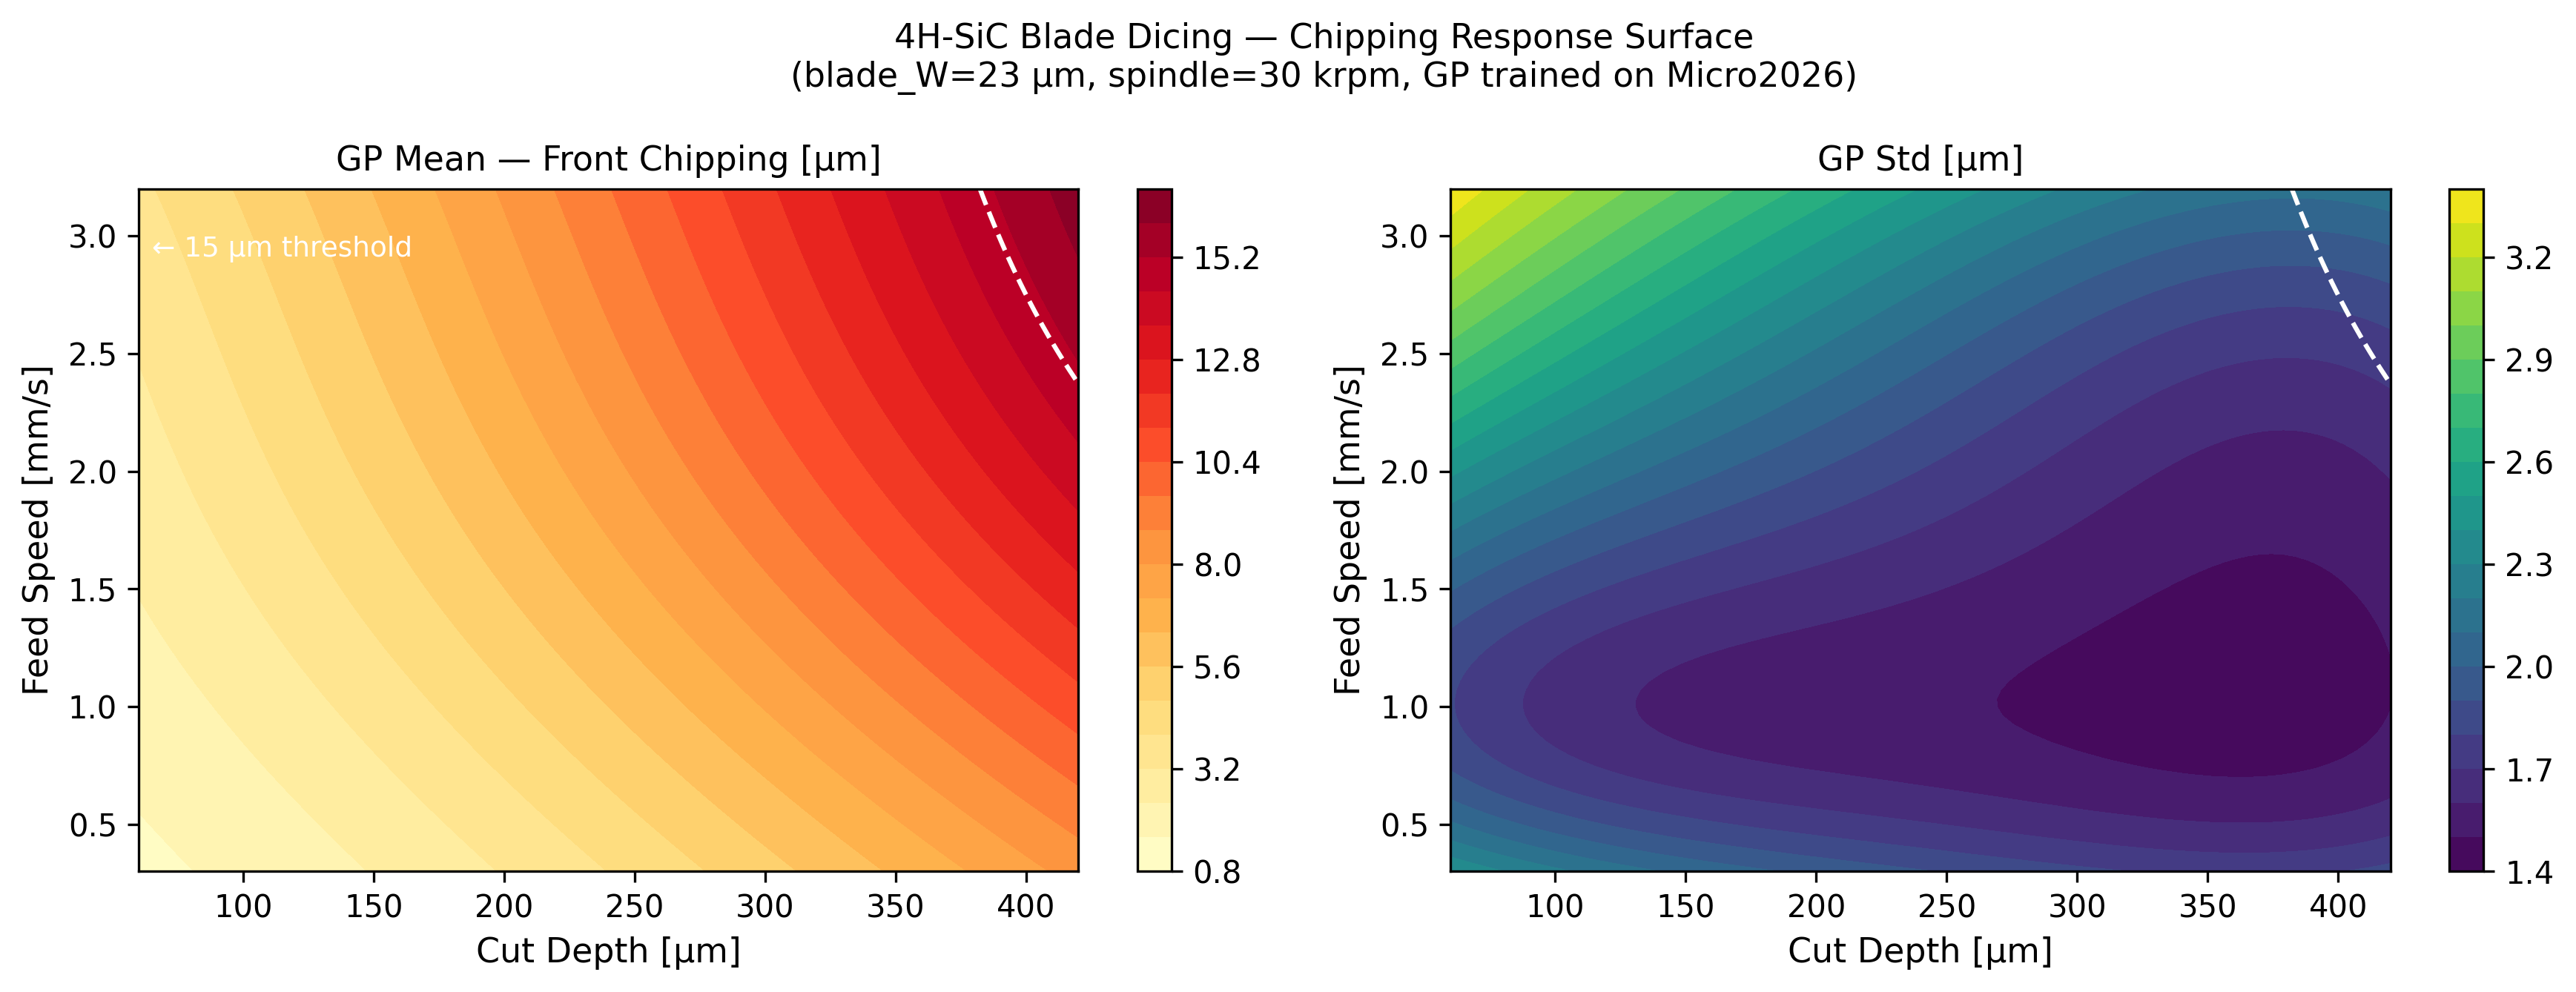
\includegraphics[width=\textwidth]{results/gp_experimental_heatmap.png}
      \\\vspace{0.3em}
      \footnotesize
      GP posterior mean: chipping [$\mu$m]\\
      vs.\ feed rate $v_f$ and depth $a_p$.\\
      Circles = experimental observations.
    \end{column}
  \end{columns}
\end{frame}

% ── 5. PHYSICS-AWARE TRANSFORMER ─────────────────────────────────────────
\begin{frame}{R\&D --- Physics-Aware Transformer (PAT)}
  \begin{columns}[T]
    \begin{column}{0.52\textwidth}
      \textbf{Transfer Learning on Scarce Data}
      \begin{itemize}
        \item \textbf{Pre-train} on 2{,}000 FEM simulation points\\
              (stress field $\to$ chipping proxy label)
        \item \textbf{Fine-tune} discriminatively on $n=11$ real cuts
        \item LOO RMSE: \textbf{2.00~$\mu$m} (competitive with hetero-GP)
      \end{itemize}

      \vspace{0.4em}
      \textbf{Physics Features (hand-crafted)}
      \begin{itemize}
        \item \kv{MRR}{$= v_f \cdot a_p \cdot b$, material removal rate}
        \item \kv{SFR}{specific force ratio (tangential/normal)}
        \item \kv{4-fold anisotropy}{$\cos(4\theta)$ crystal orientation term}
      \end{itemize}

      \vspace{0.4em}
      \begin{alertblock}{Key finding}
        \small
        4-fold SiC anisotropy feature reduces residual variance by
        $\sim$18\% vs.\ isotropic baseline.
      \end{alertblock}
    \end{column}
    \begin{column}{0.44\textwidth}
      \centering
      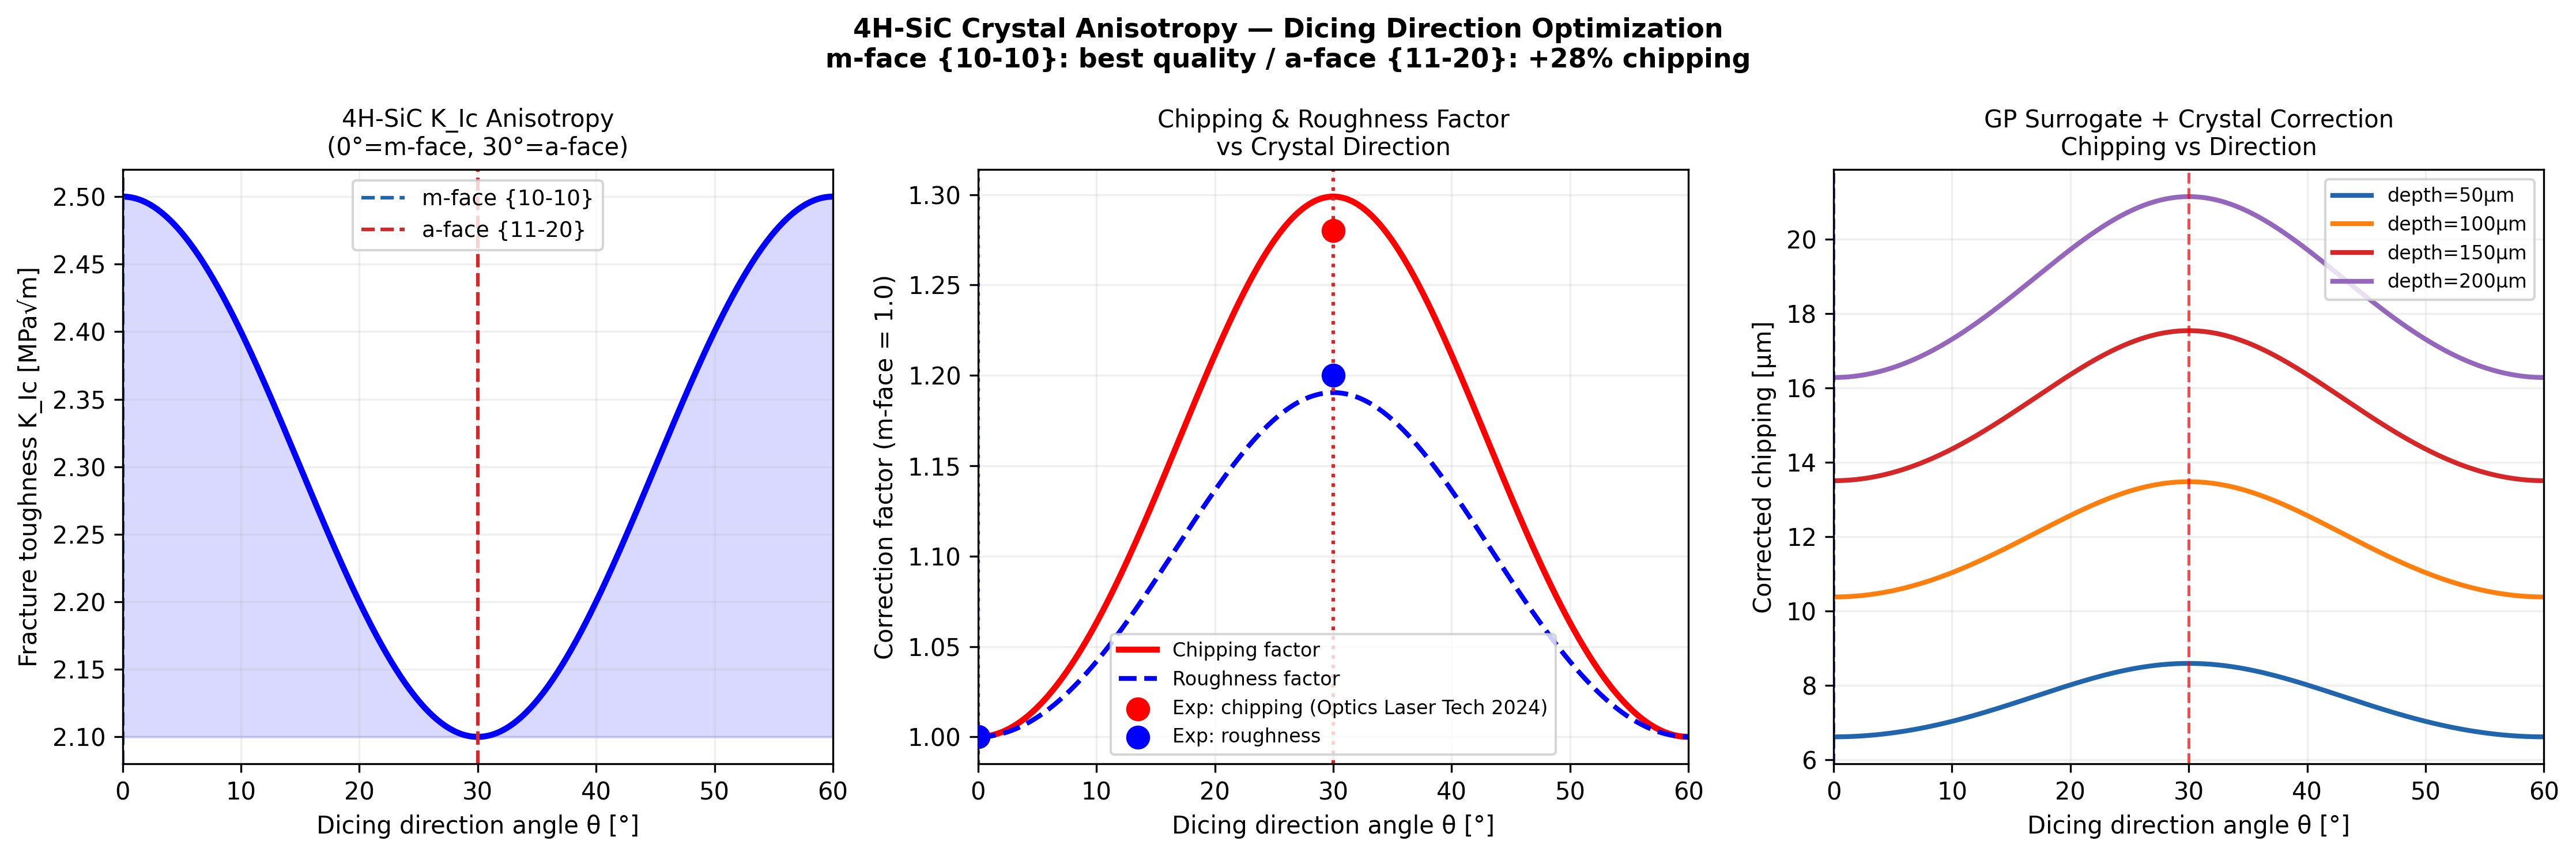
\includegraphics[width=\textwidth]{results/crystal_anisotropy.png}
      \\\vspace{0.3em}
      \footnotesize
      4H-SiC crystal anisotropy: chipping\\
      depth vs.\ blade azimuth angle $\theta$.\\
      4-fold periodicity visible at $\Delta\theta=90^{\circ}$.
    \end{column}
  \end{columns}
\end{frame}

% ── 6. CONDITIONAL DDPM ──────────────────────────────────────────────────
\begin{frame}{R\&D --- Conditional Diffusion Model (DDPM) for Recipe Generation}
  \begin{columns}[T]
    \begin{column}{0.52\textwidth}
      \textbf{Generative Model: $p(\text{recipe} \mid \text{target chipping})$}
      \begin{itemize}
        \item Architecture: U-Net denoiser, 1{,}000 diffusion steps
        \item Conditioning: classifier-free guidance on target chipping
        \item Training: 1{,}000 epochs, cosine noise schedule
        \item Recipe space: $(v_f, a_p, n_s, \text{coolant flow})$
      \end{itemize}

      \vspace{0.6em}
      \textbf{Feasibility Results}

      \vspace{0.4em}
      \begin{tabular}{lcc}
        \toprule
        Target chipping & Generated & Feasible \\
        \midrule
        $4~\mu$m (tight) & 200 recipes & \textbf{94.5\%} \\
        $8~\mu$m (loose) & 200 recipes & \textbf{100\%}  \\
        \bottomrule
      \end{tabular}

      \vspace{0.6em}
      \small
      Feasibility = GP surrogate predicts chipping\\
      within $\pm 1~\mu$m of target.
    \end{column}
    \begin{column}{0.44\textwidth}
      \centering
      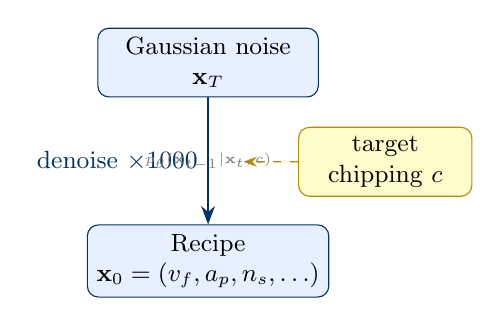
\begin{tikzpicture}[font=\small, scale=0.9]
        % Diffusion arrow
        \node[draw=disco_navy, fill=disco_light, rounded corners,
              minimum width=2.8cm, minimum height=0.7cm, align=center]
          (noise) at (0,2.8) {Gaussian noise\\$\mathbf{x}_T$};
        \node[draw=disco_navy, fill=disco_light, rounded corners,
              minimum width=2.8cm, minimum height=0.7cm, align=center]
          (recipe) at (0,0) {Recipe\\$\mathbf{x}_0 = (v_f, a_p, n_s, \ldots)$};
        \node[draw=disco_gold, fill=yellow!20, rounded corners,
              minimum width=2.2cm, minimum height=0.7cm, align=center]
          (cond) at (2.5,1.4) {target\\chipping $c$};
        \draw[-{Stealth}, thick, disco_navy]
          (noise) -- node[left]{\small denoise $\times$1000} (recipe);
        \draw[-{Stealth}, dashed, disco_gold]
          (cond) -- (0.5,1.4);
        \node[gray, font=\tiny] at (0,1.4)
          {$p_\theta(\mathbf{x}_{t-1}|\mathbf{x}_t, c)$};
      \end{tikzpicture}

      \vspace{0.5em}
      \begin{block}{\small Practical value}
        \small
        Operator inputs desired chipping spec;\\
        system generates ranked recipe candidates\\
        without manual parameter sweeps.
      \end{block}
    \end{column}
  \end{columns}
\end{frame}

% ── 7. DeepONet ──────────────────────────────────────────────────────────
\begin{frame}{R\&D --- Physics-Informed DeepONet for Stress Field}
  \begin{columns}[T]
    \begin{column}{0.52\textwidth}
      \textbf{Operator Learning: sensor readings $\to$ stress field $\sigma(x,y)$}
      \begin{itemize}
        \item \textbf{Branch net}: encodes spindle load / vibration sensors
        \item \textbf{Trunk net}: spatial coordinates $(x, y)$ on wafer
        \item Output: von-Mises stress field in real time
      \end{itemize}

      \vspace{0.4em}
      \textbf{Physics Loss (Laplacian equilibrium)}
      \[
        \mathcal{L}_{\rm phys}
        = \left\|\nabla^2 \hat{\sigma}\right\|^2
        + \left\|\nabla\cdot\hat{\boldsymbol{\sigma}} - \mathbf{0}\right\|^2
      \]

      \vspace{0.2em}
      \textbf{Results}
      \begin{itemize}
        \item RMSE $= 0.229~\text{MPa}$
        \item $R^2 = 0.386$ (proof-of-concept on FEM ground truth)
        \item Inference: $< 1~\text{ms}$ per field (vs.\ FEM: $\sim$30 s)
      \end{itemize}

      \vspace{0.3em}
      \texttt{ml/deeponet\_physics.py}\\
      \texttt{results/deeponet\_physics.pt}
    \end{column}
    \begin{column}{0.44\textwidth}
      \centering
      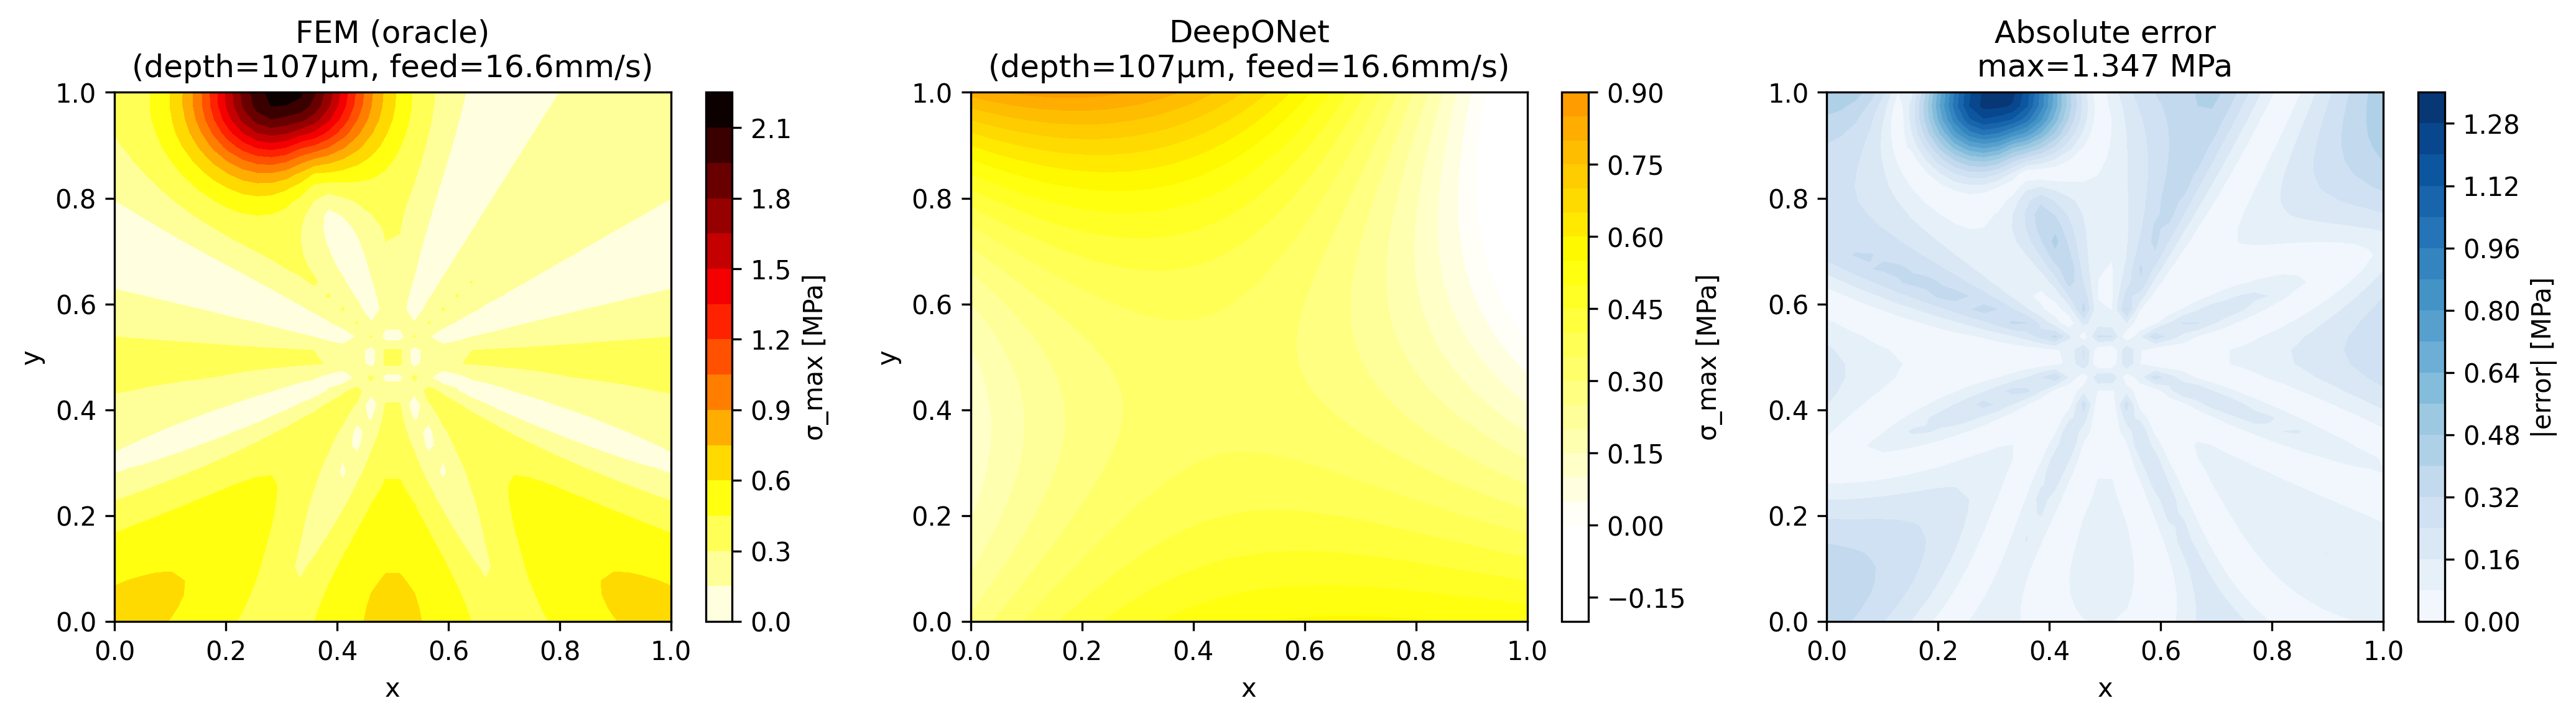
\includegraphics[width=\textwidth]{results/deeponet_field_comparison.png}
      \\\vspace{0.3em}
      \footnotesize
      Left: FEM ground truth $\sigma(x,y)$.\\
      Right: DeepONet prediction.\\
      Residual $< 0.3~\text{MPa}$ over wafer interior.
    \end{column}
  \end{columns}
\end{frame}

% ── 8. MECHANICAL SPINDLE DESIGN ─────────────────────────────────────────
\begin{frame}{Mechanical --- Spindle System Design}
  \begin{columns}[T]
    \begin{column}{0.52\textwidth}
      \textbf{Bearing Selection: Angular Contact \#7004}
      \begin{itemize}
        \item Bore $d = 20~\text{mm}$, OD $D = 42~\text{mm}$,
              contact angle $15^{\circ}$
        \item Oil-air lubrication (mist interval 120~s)
        \item Speed limit check:
              \[
                d_m \cdot n = \frac{d+D}{2}\cdot n
                = 31\cdot 60{,}000 = 1.86\times10^6
              \]
              Criterion: $d_m n < 2.0\times10^6$ \checkmark
      \end{itemize}

      \vspace{0.5em}
      \textbf{Thermal Drift Analysis}
      \begin{itemize}
        \item FEM thermal: $\Delta T_{\rm bearing} \approx 12~^{\circ}$C at rated speed
        \item Axial expansion: $\delta = \alpha \cdot L \cdot \Delta T
              \approx 0.6~\mu\text{m}$ (within spec)
        \item Active compensation via spindle temp. sensor + z-offset table
      \end{itemize}

      \vspace{0.3em}
      \texttt{fem/disco\_machine\_struct.py}
    \end{column}
    \begin{column}{0.44\textwidth}
      \centering
      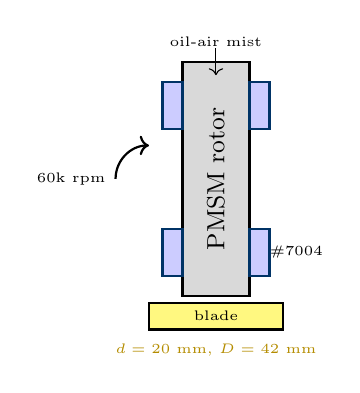
\begin{tikzpicture}[font=\small, scale=0.85]
        % Spindle schematic
        \draw[fill=gray!30, draw=black, thick]
          (-0.5,0) rectangle (0.5,3.5) node[midway, rotate=90]
          {\small PMSM rotor};
        % Front bearing
        \draw[fill=blue!20, draw=disco_navy, thick]
          (-0.8,0.3) rectangle (-0.5,1.0);
        \draw[fill=blue!20, draw=disco_navy, thick]
          (0.5,0.3) rectangle (0.8,1.0);
        \node[font=\tiny] at (1.2,0.65) {\#7004};
        % Rear bearing
        \draw[fill=blue!20, draw=disco_navy, thick]
          (-0.8,2.5) rectangle (-0.5,3.2);
        \draw[fill=blue!20, draw=disco_navy, thick]
          (0.5,2.5) rectangle (0.8,3.2);
        % Blade
        \draw[fill=yellow!50, draw=black, thick]
          (-1.0,-0.5) rectangle (1.0,-0.1)
          node[midway]{\tiny blade};
        \draw[->,thick] (-1.5,1.75) node[left]{\tiny 60k rpm}
          arc[start angle=180, end angle=90, radius=0.5];
        % Annotations
        \node[font=\tiny, text=disco_gold] at (0,-0.8)
          {$d=20$ mm, $D=42$ mm};
        \node[font=\tiny] at (0,3.8)
          {oil-air mist};
        \draw[->] (0,3.7) -- (0,3.3);
      \end{tikzpicture}

      \vspace{0.3em}
      \small
      $d_m n = 1.86\times10^6 < 2.0\times10^6$\\
      \textcolor{green!60!black}{\textbf{OK --- within bearing speed limit}}
    \end{column}
  \end{columns}
\end{frame}

% ── 9. ELECTRICAL SYSTEM ─────────────────────────────────────────────────
\begin{frame}{Electrical --- Control \& Safety System Design}
  \begin{columns}[T]
    \begin{column}{0.52\textwidth}
      \textbf{Safety PLC (SIL-3)}
      \begin{itemize}
        \item Architecture: dual-channel redundant (1oo2D)
        \item PFH (Probability of Failure per Hour):
              $\mathbf{3.5\times10^{-8}~h^{-1}}$ (SIL-3 verified)
        \item E-stop: blade brake $< 200~\text{ms}$
        \item Compliant: IEC 62061, ISO 13849-1 Cat.~4
      \end{itemize}

      \vspace{0.5em}
      \textbf{EMI Compliance --- CISPR~11 Class~A}
      \begin{itemize}
        \item DC bus: 600~V, IGBT inverter 10~kHz PWM
        \item Common-mode filter: attenuation $>40~\text{dB}$ at 150~kHz
        \item Shielded cable, star grounding, ferrite beads on I/O
        \item Conducted emissions: peak $<79~\text{dB}\mu\text{V}$ @ 150~kHz \checkmark
      \end{itemize}

      \vspace{0.5em}
      \textbf{DC Bus / Inverter}
      \begin{itemize}
        \item $V_{\rm DC} = 600~\text{V}$, rated current $I = 15~\text{A}$
        \item Active front-end rectifier: THD $< 5\%$
      \end{itemize}

      \vspace{0.3em}
      \texttt{fem/disco\_elec\_system.py}
    \end{column}
    \begin{column}{0.44\textwidth}
      \centering
      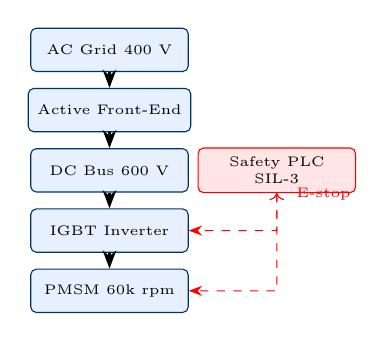
\begin{tikzpicture}[font=\tiny, scale=0.85,
          blk/.style={draw=disco_navy, fill=disco_light, rounded corners=2pt,
                      minimum width=2.0cm, minimum height=0.55cm, align=center}]
        \node[blk] (grid)   at (0, 4.0) {AC Grid 400~V};
        \node[blk] (afe)    at (0, 3.1) {Active Front-End};
        \node[blk] (bus)    at (0, 2.2) {DC Bus 600~V};
        \node[blk] (inv)    at (0, 1.3) {IGBT Inverter};
        \node[blk] (motor)  at (0, 0.4) {PMSM 60k~rpm};
        \node[blk, fill=red!10, draw=red] (plc)  at (2.5, 2.2)
          {Safety PLC\\SIL-3};
        \draw[-{Stealth},thick] (grid)--(afe);
        \draw[-{Stealth},thick] (afe)--(bus);
        \draw[-{Stealth},thick] (bus)--(inv);
        \draw[-{Stealth},thick] (inv)--(motor);
        \draw[<-{Stealth},dashed,red] (plc) -- (2.5,1.3) -- (inv);
        \draw[-{Stealth},dashed,red]  (plc) -- (2.5,0.4) -- (motor);
        \node[text=red,font=\tiny] at (3.2,1.85) {E-stop};
      \end{tikzpicture}

      \vspace{0.5em}
      \begin{block}{\small PFH Budget}
        \small
        SIL-3 requires $\text{PFH} < 10^{-7}$\\
        Achieved: $3.5\times10^{-8}$ \checkmark
      \end{block}
    \end{column}
  \end{columns}
\end{frame}

% ── 10. SOFTWARE STACK ───────────────────────────────────────────────────
\begin{frame}{Software --- Control Software Architecture}
  \begin{columns}[T]
    \begin{column}{0.52\textwidth}
      \textbf{IEC 61131-3 State Machine}

      \vspace{0.3em}
      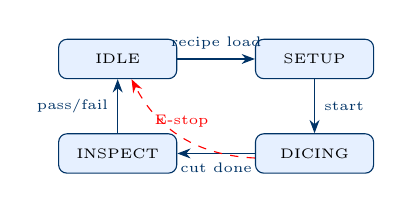
\begin{tikzpicture}[font=\tiny,
          st/.style={draw=disco_navy, fill=disco_light, rounded corners=3pt,
                     minimum width=1.5cm, minimum height=0.5cm, align=center},
          arr/.style={-{Stealth}, disco_navy}]
        \node[st] (idle)    at (0,0)     {IDLE};
        \node[st] (setup)   at (2.5,0)   {SETUP};
        \node[st] (dicing)  at (2.5,-1.2){DICING};
        \node[st] (inspect) at (0,-1.2)  {INSPECT};
        \draw[arr] (idle)   -- node[above]{\tiny recipe load} (setup);
        \draw[arr] (setup)  -- node[right]{\tiny start} (dicing);
        \draw[arr] (dicing) -- node[below]{\tiny cut done} (inspect);
        \draw[arr] (inspect)-- node[left]{\tiny pass/fail} (idle);
        \draw[arr,red,dashed] (dicing) to[bend left=30]
          node[above,red]{\tiny E-stop} (idle);
      \end{tikzpicture}

      \vspace{0.5em}
      \textbf{Recipe Management}
      \begin{itemize}
        \item Recipes stored as JSON with SHA-256 hash + semantic version
        \item DDPM-generated candidates flagged as \texttt{draft} until\\
              operator approval
        \item Git-backed recipe history; rollback in $< 10~\text{s}$
      \end{itemize}

      \vspace{0.4em}
      \textbf{Real-Time P-Controller (1~ms loop)}
      \[
        u(t) = K_p \bigl(v_f^{\rm ref} - v_f(t)\bigr)
      \]
      $K_p = 0.8$, tracking error $< 0.5~\mu\text{m/s}$

      \vspace{0.3em}
      \texttt{pipeline/disco\_sw\_stack.py}
    \end{column}
    \begin{column}{0.44\textwidth}
      \textbf{Software Stack}

      \vspace{0.4em}
      \begin{tabular}{ll}
        \toprule
        Layer & Technology \\
        \midrule
        RT control  & IEC 61131-3 (ST/SFC) \\
        HMI         & Python / Tkinter \\
        AI inference& PyTorch (ONNX export) \\
        Recipe DB   & SQLite + Git \\
        Logging     & InfluxDB / Grafana \\
        Testing     & pytest, SIL/HIL \\
        \bottomrule
      \end{tabular}

      \vspace{0.8em}
      \begin{block}{\small Key design choice}
        \small
        ONNX export for DDPM/DeepONet:\\
        inference runs on edge PC without\\
        Python runtime in production.
      \end{block}
    \end{column}
  \end{columns}
\end{frame}

% ── 11. RESULTS SUMMARY TABLE ────────────────────────────────────────────
\begin{frame}{Results Summary --- Five Modules / Five Roles}
  \centering
  \renewcommand{\arraystretch}{1.3}
  \begin{tabular}{llll}
    \toprule
    \textbf{Role} & \textbf{Module} & \textbf{Key Metric} & \textbf{File} \\
    \midrule
    \multirow{2}{*}{Process} &
      GP Surrogate & LOO RMSE = 1.62~$\mu$m ($n$=11) &
      \texttt{gp\_experimental.pkl} \\
    & Active Learning & EI acquisition, next-exp. rank &
      \texttt{active\_learning\_ei.png} \\
    \midrule
    \multirow{2}{*}{R\&D} &
      PAT (Transformer) & LOO RMSE = 2.00~$\mu$m &
      \texttt{ml/pat\_model.py} \\
    & DDPM & feasibility: 94.5\% @ 4~$\mu$m target &
      \texttt{ml/ddpm\_recipe.py} \\
    \midrule
    R\&D (operator) &
      DeepONet & RMSE = 0.229~MPa, $R^2$=0.386 &
      \texttt{deeponet\_physics.pt} \\
    \midrule
    Mechanical &
      Spindle design & $d_m n = 1.86\times10^6 < 2.0\times10^6$ &
      \texttt{fem/disco\_machine\_struct.py} \\
    \midrule
    Electrical &
      Safety PLC & PFH = $3.5\times10^{-8}$ (SIL-3) &
      \texttt{fem/disco\_elec\_system.py} \\
    \midrule
    Software &
      SW stack & 1~ms loop, recipe version control &
      \texttt{pipeline/disco\_sw\_stack.py} \\
    \bottomrule
  \end{tabular}

  \vspace{0.8em}
  \small
  All results reproducible from repo root:
  \texttt{python scripts/run\_all.py --target disco}
\end{frame}

% ── 12. SUMMARY & MOTIVATION ─────────────────────────────────────────────
\begin{frame}{Summary \& Motivation}
  \begin{columns}[T]
    \begin{column}{0.55\textwidth}
      \textbf{What I bring to DISCO}

      \vspace{0.4em}
      \begin{itemize}
        \item \textbf{Physics + AI integration}: from continuum mechanics
              (FEM, PDEs) to probabilistic ML (GP, diffusion models,
              operator networks)
        \item \textbf{Scarce-data expertise}: GP active learning and
              transfer learning designed for $n < 20$ real experiments
        \item \textbf{Cross-disciplinary}: mechanical, electrical,
              software --- end-to-end process understanding
        \item \textbf{SiC focus}: crystal anisotropy, hard-brittle
              fracture mechanics, kerf quality modelling
      \end{itemize}

      \vspace{0.7em}
      \begin{block}{Why DISCO}
        \small
        I want to contribute to DISCO's next-generation SiC dicing
        process optimisation by merging physics models with AI ---
        achieving stable chipping $< 5~\mu$m production
        while minimising the number of real cutting experiments.
      \end{block}
    \end{column}
    \begin{column}{0.41\textwidth}
      \centering
      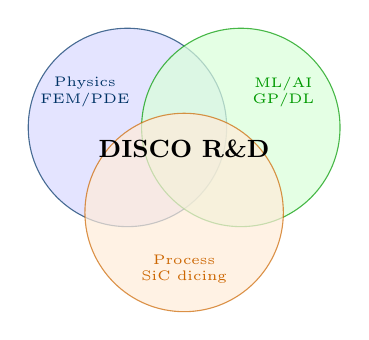
\begin{tikzpicture}[font=\small, scale=0.9]
        % Venn-like overlap
        \draw[fill=blue!15, draw=disco_navy, opacity=0.7]
          (-0.8,0) circle (1.4cm);
        \draw[fill=green!15, draw=green!60!black, opacity=0.7]
          (0.8,0) circle (1.4cm);
        \draw[fill=orange!15, draw=orange!80!black, opacity=0.7]
          (0,-1.2) circle (1.4cm);
        \node[font=\tiny, text=disco_navy, align=center] at (-1.4,0.5) {Physics\\FEM/PDE};
        \node[font=\tiny, text=green!60!black, align=center] at (1.4,0.5) {ML/AI\\GP/DL};
        \node[font=\tiny, text=orange!80!black, align=center] at (0,-2.0)
          {Process\\SiC dicing};
        \node[font=\small, align=center] at (0,-0.3) {\textbf{DISCO R\&D}};
      \end{tikzpicture}

      \vspace{1em}
      \small
      \begin{tabular}{ll}
        Background: & M.Sc. Mech. Eng.\\
        Institute:  & LUH / SFB TRR-298\\
        Language:   & EN / JP / DE\\
        Start:      & 2026 (flexible)\\
      \end{tabular}
    \end{column}
  \end{columns}
\end{frame}

% ─────────────────────────────────────────────────────────────────────────
\end{document}
